\begin{figure}[!htbp]
\begin{center}

\begin{minipage}{\linewidth}
\begin{subfigure}[b]{\linewidth}
\begin{minipage}{0.5\textwidth}
\begin{center}
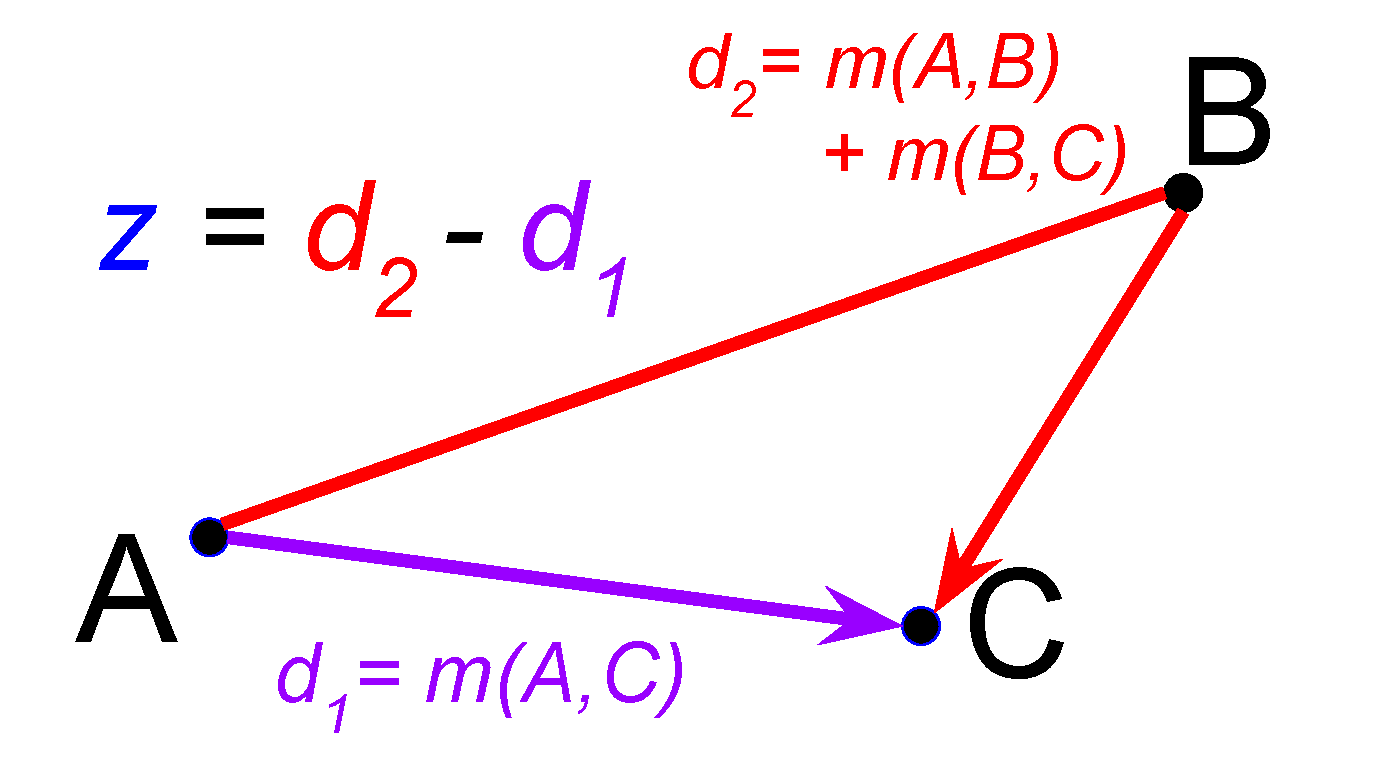
\includegraphics[width=\linewidth]{img/detour-difference}
\end{center}
\end{minipage}%
\begin{minipage}{0.5\textwidth}
\caption{
Sampling process used to evaluate detour difference, $z$.
} \label{fig:detour_difference_cartoon}
\end{minipage}
\end{subfigure}
\end{minipage}

\begin{minipage}{\linewidth}
\begin{subfigure}[b]{\linewidth}
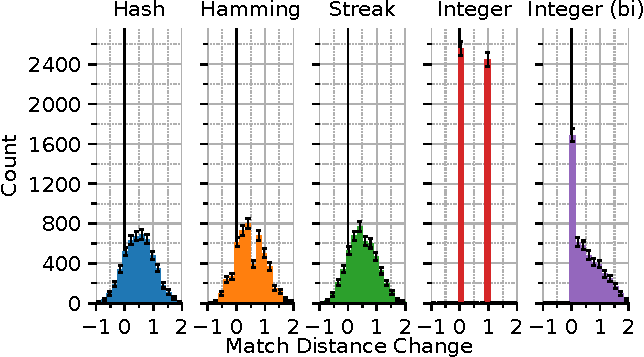
\includegraphics[width=\linewidth]{img/detour_difference/bitweight=0dot5+seed=1+title=low-triplet-analysis+viz=hist+_data_hathash_hash=6b0749ef97a58721+_script_fullcat_hash=ab23ac25d229f726+ext=}
\caption{
Distributions of detour distance difference for triplets of randomly sampled tags.
Positive values indicate that total distance increased with the addition of an intermediate stop.
A value of exactly 0 indicates an intermediate stop had no effect on total distance.
Negative values indicate violation of the triangle inequality: taking an intermediate stop reduced the total distance traveled.
Error bars are 95\% confidence intervals calculated using the Wilson score method with continuity correction \citep{newcombe1998two}.
} \label{fig:detour_difference_distribution}

\end{subfigure}
\end{minipage}

\caption{
Detour difference of tag-matching metrics.
Supplementary Figure \ref{fig:uniformification_supp} shows the cumulative distribution of all sampled detour difference values for each metric.
}
\label{fig:detour_difference}

\end{center}
\end{figure}
